\فصل{روش $Ziggurate$}
\section{معرفی}

در روش زیگورات تلاش است تا یک مصالحه بین زمان و حافظه ایجاد کند. این روش به برنامه‌نویس این امکان را می‌دهد که خود انتخاب کند چه میزان از حافظه خود را صرف ذخیره‌سازی اعداد از پیش محاسبه‌شده بکند. 
\\
در الگوریتم زیگورات از مستطیل‌های از پیش محاسبه شده استفاده می‌شود که دارای "اندازه" یکسان برای پرکردن فضای زیر تابع چگالی احتمال $(PDF)$، می‌باشد. زیادکردن تعداد مستطیل‌ها سرعت را افزایش می‌دهد و از سویی استفاده از حافظه را بیشتر می‌کند. بنابراین کنترل مصالحه به عهده کاربر این الگوریتم است. به طور مثال در دستگاه‌هایی مانند کارت‌های هوشمند و میکروکنترلرها که حافظه محدودی دارند، باید به سرعت کمتری تن داد در حالی که در دستگاه‌هایی که حافظه بیشتری دارند می توان از سرعت‌های بالاتری برخوردار بود. الگوریتم زیگورات برای توزیع پیوسته طراحی شده‌است اما می‌توان با درنظر گرفتن نکاتی از آن برای توزیع‌های گسسته استفاده کرد. برای این کار باید واژه "اندازه" برای یک مستطیل  باید از مفهوم "مساحت" به مفهوم عمده " احتمال قرار گرفتن نقاط نمونه درون مستطیل " تغییر پیدا کند. 
\\
الگوریتم زیگورات از رده الگوریتم‌های نمونه‌برداری ردی است و توسط $Marsaglia$  و $Tsang$  برای نمونه‌برداری پیوسته توزیع گوسی معرفی شد. 
  
در این الگوریتم ما می‌خواهیم از توزیع گوسی که میانه آن صفر و دامنه ی مورد بحث $B :=[-t_{\sigma}, t_{\sigma}]\cap \mathbb{Z}$   است استفاده کنیم. دامنه$t$ به اندازه کافی  برای  استفاده در رمزنگاری مشبکه مبنا بزرگ انتخاب می‌شود. در این‌جا توزیع پیرامون نقطه صفر است، اما می‌توان یک عدد ثابت را به نمونه‌ها اضافه کرد و به این صورت می‌توان نمودار را پیرامون هر عدد غیر صفر داشت.
\\
می‌توان از قسمت مثبت نمونه‌برداری کرد و همین نمونه‌برداری را برای قسمت منفی متناظر کرد. اگر عدد برگردانده‌شده از الگوریتم $x = 0$ باشد، این عدد را با احتمال $\frac{1}{2}$ قبول می‌کنیم در غیر این صورت از میان $s\in \lbrace -1, 1\rbrace $ یک عدد انتخاب می‌کنیم و عدد نهایی که برگردانده‌می‌شود $sx$ می باشد.
\section{نمونه برداری در فضای مثبت }

در این روش از تابع چگالی احتمال $(PDF)$ استفاده می‌شود.  تابع $(PDF)$ را به یک فضا به نام $A$  که شامل $m$ مستطیل افقی است که مساحت‌های برابری دارند، تبدیل می‌کنیم. همان‌طور که در شکل\ref{Ziggurate-intro} نشان داده‌شده‌است.

    \begin{figure}[!htb]
      	\centering
      	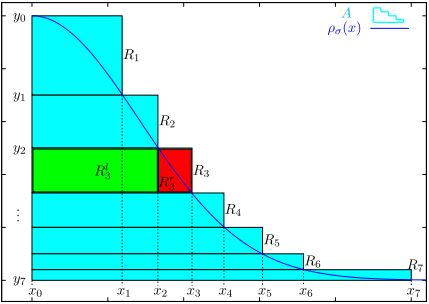
\includegraphics[scale=0.6]{images/Ziggurate-intro.eps}
      	\caption{روش زیگورات با 7 مستطیل و سطح پوشیده‌شده A}
      	\label{Ziggurate-intro}


      \end{figure}

یک جفت عدد $(x_{i},y{i})$ که نشان‌دهنده گوشه پایین مستطیل $R_{i}$ است ،$1< i < m - 1$، را نگه می‌داریم. 
هر مستطیل را می‌توان به دو مستطیل  سمت راست$ R^{r}_{i}$ و  سمت چپ$ R^{l}_{i}$ تقسیم کرد. مستطیل سمت چپ به طور کامل زیر نمودار $PDF$گوسی قرار دارد و مستطیل سمت راست تا حدودی زیر نمودار $PDF$  قرار دارد. می‌توان برای نمونه به $R_{6}$  در شکل \ref{Ziggurate-intro} نگاه کرد.
\\
برای این‌که بتوان نمونه $x \leq t_{\sigma}$  در $\mathbb{R}^{+}_{0}$  انتخاب کرد ، ابتدا برای انتخاب یک مستطیل ،یک عدد $1 \leq i \leq m$ را به صورت یکنواخت انتخاب می‌کنیم.  سپس یک $ x$  درون $R_{i}$ به صورت یکنواخت  از  $[0, x_{i}]$ انتخاب می کنیم  و آن را $x'$  می‌نامیم. اگر$ x’\leq   x_{i – 1}$   در این صورت  $x'$   درون $ R^{l}_{i}$ قرار دارد مستقیما این عدد را به عنوان خروجی برمی‌گردانیم، در غیر این صورت$x'$  در$ R^{r}_{i}$ واقع شده است. در این شرایط ما از نمونه‌برداری ردی استفاده می‌کنیم. یک نمونه همانند $\gamma$  در بازه $ [y_{i+1}, y_{i}]$ به صورت یکنواخت انتخاب می‌کنیم. سپس اگر $\gamma \leq \rho _{\sigma (x')}$ یک عدد از زیر نمودار انتخاب کرده‌ایم،   $x'$ را انتخاب می‌کنیم و برمی‌گردانیم. در غیر این صورت نمونه را رد می کنیم و دوباره تمام مراحل را  با نمونه‌ جدید $i$  تکرار می‌کنیم.
\\
این الگوریتم در واقع همان الگوریتم نمونه‌برداری ردی است که قسمت اول الگوریتم (نمونه برداری یک نقطه در فضای زیر نمودار) بهتر شده‌است. در این روش تمام مستطیل ها سایز برابر دارند بنابراین احتمال آن‌که نقطه انتخاب‌شده در هرکدام از  مستطیل‌ها باشد برابر است. بنابراین می توان ابتدا از بین مستطیل‌ها نمونه برداری کرد و سپس یک نقطه در مستطیل‌ها انتخاب کرد.
\\
بیشترین هزینه این الگوریتم‌ در محاسبه$\rho_{\sigma}(x')$  است، زمانی که  $x'$ در مستطیل$ R^{l}_{i}$ واقع نشده‌باشد.  اگر این نمونه رد شود هزینه بیشتری دارد. بنابراین زیگورات یک مصالحه بین زمان و حافظه است که به وسیله تعداد مستطیل‌ها کنترل می‌شود. اگر تعداد بیشتری مستطیل استفاده کنیم، نسبت بین مستطیل  چپ و راست تغییر می‌کند به طوری که نسبت مستطیل چپ نسبت به مستطیل راست ، بزرگتر می‌شود. بنابراین با احتمال بیشتری می‌توان  یک $x'$ را بدون محاسبه$\rho_{\sigma}(x')$    پذیرفت.همچنین در صورتی که تعداد مستطیل‌ها زیادتر شود فضای$ A$  به فضای $C$   که زیر $PDF$ نزدیک‌تر است. در نتیجه میزان نمونه‌‌هایی که رد می‌شوند کاهش می‌یابد. اما برای هر مستطیل اضافی باید نقاط مرتبط با این مستطیل  که محل مستطیل‌ها را در  صفحه نشان‌می‌دهد، نگه‌داری شود بنابراین به استفاده بیشتر از حافظه نیاز دارد.
\section{تغییر الگوریتم برای فضای گسسته}
در فضای گسسته نیز الگوریتم مانند قبل عمل می‌کند.  در این حالت نیز علامت $s$، مستطیل‌های با نمایه $i$ و نمونه‌های $x'$ را داریم. اگر $ x'$  در قسمت چپ مستطیل واقع شده‌باشد و صفر نباشد $sx'$ برگردانده می‌شود.  اگر $x'$ برابر صفر شد،  همانند حالت پیوسته، با احتمال $\frac{1}{2}$ برگردانده می‌شود. اگر $x'$ غیر از صفر باشد  دقیقا همانند حالت پیوسته از نمونه‌برداری ردی استفاده می‌شود و تصمیم گرفته می‌شود که $sx'$ برگردانده شود یا دورریخته شود و دوباره پردازش انجام گیرد.
\\ 
تفاوتی که در فضای گسسته وجود دارد، نمی‌توان از کلمه "اندازه " \پانوشت{\متن‌لاتین {size} } برای مساحت‌های مستطیل در حالت گسسته استفاده کرد. اندازه‌های مستطیل باید متناسب احتمال نمونه‌برداری یک نقطه که در این فضا هست، باشد.  بنابراین در حالت گسسته اندازه مستطیل به صورت حاصل ضرب تعداد $x$ های صحیح که در بازه مربوطه قرار دارد ضربدر ارتفاع مستطیل تعریف می‌شود . به طور مثال ،  اندازه مستطیل $R_{3}$  برابر $(1 + \lfloor x_{3}\rfloor ).(y_{2} - y_{3}) $ می‌باشد.
\\
دومین اختلاف میان حالت گسسته و پیوسته در روش محاسبه مستطیل‌ها است.  برای حالت پیوسته محاسبه آن‌ها از حیطه بحث خارج است . برای حالت گسسته الگوریتم زیگورات نشان می‌دهیم که چگونه قسمت‌بندی‌ها را انجام دهیم تا $m$ مستطیل با اندازه برابر داشته باشیم . بنابراین داریم :
\begin{equation}
y_{m} := 0, 		x_{0} := 0,		x_{m} := t_{\sigma},
\end{equation} 
 و سایر قسمت‌بندی ها را از " راست به چپ از طریق زیر پیدا می‌کنیم.
    
     \begin{align*}
     y_{m-1} = \frac{S}{1+\lfloor x_{m}\rfloor}, &\quad &\quad x_{m-1}=\rho ^{-1}_{\sigma},\\
     \quad
     for i = m-2,...,1:	 &\quad y_{i}=\frac{S}{1+\lfloor x_{i+1}\rfloor}+y_{i+1}, &\quad & x_{i} = \rho ^{-1}_{\sigma}(y_{1}),
     \\ \quad
     y_{0}= \frac{S}{1+\lfloor x_{1}\rfloor} + y_{1}.
          \end{align*}
   

      
   \section{بهبود روش }   
با توجه به اینکه بیشترین وقتی که در الگوریتم زیگورات صرف می‌شود، مربوط به محاسبه $\rho _{\sigma}$ می‌باشد بنابراین برای بهبود باید تا آنجایی که ممکن است از محاسبه آن اجتناب شود. $\rho _{\sigma}$ زمانی نیاز است که $(x,y)$ در قسمت راست مستطیل $R^{r} _{i}$ واقع شده‌باشد. اما در این شرایط با توجه به این‌که $\rho _{\sigma}$  که درون $R^{r} _{i}$چه شکلی دارد، می‌توان از حساب کردن $\rho _{\sigma}$ در نصف مواقع جلوگیری کرد و راحتتر $x$ را قبول یا رد کرد.
\\
ما $R^{r} _{i}$ را با وصل کردن بالا چپ به پایین راست با خط راست $s$ قسمت می‌کنیم. $\rho _{\sigma}$   دارای نقطه عطف است که در قسمت مثبت نمودار، قبل از نقطه عطف تقعر نمودار به سمت پایین است و بعد از نقطه عطف تقعر نمودار به سمت بالا است (شکل  \ref{ZiggurateO})   $x$ که انتخاب می‌شود اگر کمتر از نقطه عطف باشد همه نقاط $(x,y)$ در مستطیل $R^{r} _{i}$که زیر خط $s$ قرار می‌گیرند، پذیرفته می‌شوند و $x$ به عنوان خروجی برگردانده می‌شود. در جایی که تقعر نمودار به سمت بالا است (بعد از نقطه عطف )همه نقاط بالای $s$ به سرعت رد می‌شود. در سایر شرایط $\rho _{\sigma}$ باید محاسبه شود و شرایط پذیرفتن چک شود. برای روش زیگورات در حالت گسسته باید به جای $x_{i}$ از $\lfloor x_{i}\rfloor $ استفاده شود. این روش را با $ZiggurateO$  نشان می دهیم\cite{510}.
    \begin{figure}[!htb]
      	\centering
      	\includegraphics[scale=0.45]{images/Ziggurate-concave.eps}
      	\caption{الگوریتم  بهبود یافته زیگورات برای نمونه‌برداری گسسته}

		\label{ZiggurateO}
      \end{figure}
      

